\documentclass[tikz,border=12pt]{standalone}
\begin{document}
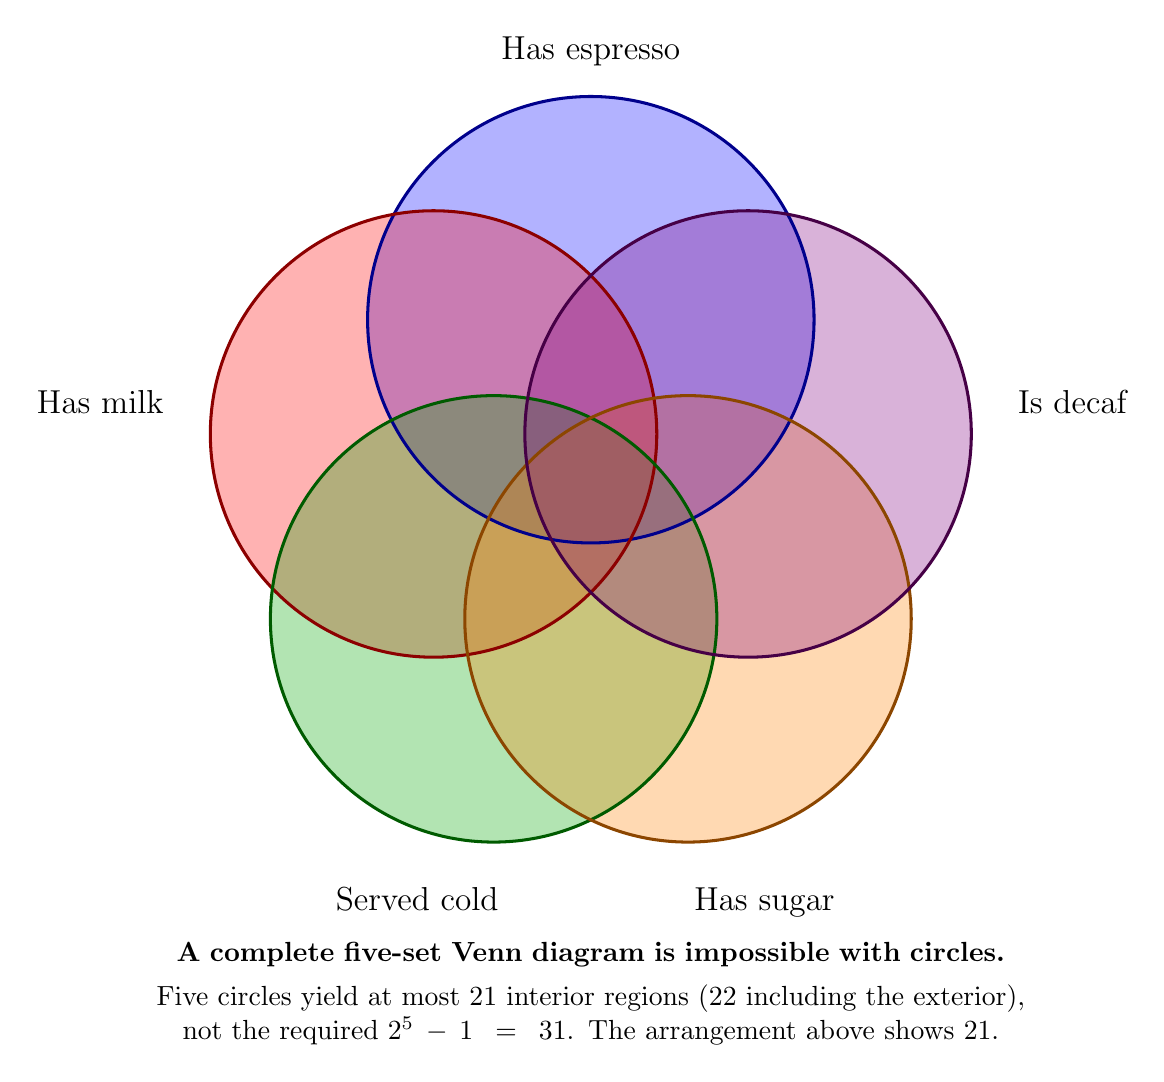
\begin{tikzpicture}[scale=1.05]
  % pentagon circumradius and circle radius
  \def\d{2}
  \def\r{2.7}
  % the five circles, centres on a regular pentagon
  \foreach \a/\c in {90/blue, 162/red, 234/green!65!black, 306/orange, 18/violet}{
    \fill[\c, opacity=0.30] (\a:\d) circle (\r);
  }
  % Draw outlines after all fills so every boundary remains crisp.
  \foreach \a/\c in {90/blue, 162/red, 234/green!65!black, 306/orange, 18/violet}{
    \draw[\c!55!black, line width=1.1pt] (\a:\d) circle (\r);
  }
  % labels
  \node[font=\large, anchor=south] at (0, 4.95)     {Has espresso};
  \node[font=\large, anchor=east]  at (-5.05, 1.0)  {Has milk};
  \node[font=\large, anchor=north] at (-2.1, -4.75) {Served cold};
  \node[font=\large, anchor=north] at (2.1, -4.75)  {Has sugar};
  \node[font=\large, anchor=west]  at (5.05, 1.0)   {Is decaf};
  \node[align=center, text width=13cm, font=\normalsize] at (0,-6.15)
    {\textbf{A complete five-set Venn diagram is impossible with circles.}\\[4pt]
     Five circles yield at most 21 interior regions (22 including the exterior),\\
     not the required $2^5-1=31$. The arrangement above shows 21.};
\end{tikzpicture}
\end{document}
